\documentclass{../../oss-handout}
\usepackage{amsmath}
\usepackage{newtxtext,newtxmath}
\usepackage{enumitem}
\usepackage{tikz}
\usepackage{siunitx}
\usepackage{xcolor,colortbl}
\usepackage{cancel}
\usepackage{wrapfig}
\usepackage{textcomp}

\sisetup{
  per-mode=symbol
}

\setlength{\parindent}{0pt}
\setlength{\parskip}{6pt}
\setlength{\headheight}{26pt}

\newcommand{\pic}[2]{\includegraphics[width=#1\textwidth]{#2}}

% Set the page style for the document
\pagestyle{plain}

% Course & handout information
\renewcommand{\institution}{Olympiads School, Toronto, Ontario, Canada}
\renewcommand{\coursetitle}{Grade 12 Physics}
\renewcommand{\term}{Updated: Fall 2022}
\title{Uncertainties and Significant Figures}
\author{Dr.\ Timothy Leung}
\date{\today}

\begin{document}
\thispagestyle{title}
\gentitle

There are things that we must learn\footnote{Or in this case, be reminded of!}
\emph{before} we do any physics. Understanding how measurements are made and
how to deal with inaccuracies in numbers is fundamentally important in all
branches of science. This handout is also given in Physics 11. If you already
have a copy from previous classes, then this is exactly the same.

\begin{center}
  \textbf{Counting vs.\ Measuring vs.\ Estimating}
\end{center}

Some physical quantities can be \textbf{counted} exactly. These quantities have
\emph{discrete} values (whole numbers or integers) that are expressed
\emph{exactly} with \emph{no uncertainties}. They are usually expressed as
integers or fractions (rational numbers). For example:
\begin{itemize}[nosep]
\item There are 30 students and one teacher in this classroom
\item $\dfrac{13}{30}$ of the Grade 12 Physics students are girls (both the
  number of girls and the total number of students are counted exactly)
\item There are two engines on a Boeing 777 aircraft (shown in
  Figure~\ref{fig:count})
\item My brother owes me \$ 2.45 (exactly 245 \textcent)
\end{itemize}
\begin{figure}[ht]
  \centering
  \pic{.45}{../graphics/1552937371896}
  \caption{The number of engines on an airplane can be counted exactly.}
  \label{fig:count}
\end{figure}

However,this is not the case with numbers that are \textbf{measured}, which
include most physical quantities that we encounter in science. For example:
\begin{itemize}[nosep]
\item The volume of blue liquid in a graduated cyliner is \SI{74}{\milli\litre}
  (Figure~\ref{fig:cylinder})
\item The distance between Toronto and Montreal is \SI{545}{\kilo\metre}.
\item The car is moving at a velocity of \SI{45.4}{\metre\per\second} [west].
\item A tow truck is pulling a car using \SI{4500}{\newton} of force.
\item The frequency of sound from an out-of-tine violin string is
  \SI{441.5}{\hertz}.
\item The sound intensity of a jet engine during take-off is \SI{121}{dB}
  from \SI{5.}{\metre} away.
\end{itemize}
\begin{figure}[ht]
  \centering
  \pic{.4}{../graphics/graduated-cylinder}
  \caption{What is the reading on this graduated cylinder?}
  \label{fig:cylinder}
\end{figure}

Measured quantities are usually \emph{continuous} variables that are best
expressed with decimals. A measured quantity will always have \emph{some}
uncertainties, depending on:
\begin{itemize}[nosep]
\item Uncertainties in the tools used to make the measurements
\item Errors introduced by the person making the measurements, etc
\end{itemize}
There are also numbers which are (usually) too large to be counted, and are
therefore \textbf{estimated} instead. For example:
\begin{itemize}[nosep]
\item There are 7.714 billion people on Earth
\item A bag of popcorn contains 600 kernels of popcorn
  (Figure~\ref{fig:popcorn})
\end{itemize}
In these estimates, the exact values are usually not the most important
(otherwise some poor graduate students at a university would be told by their
professors to count exactly); we treat them the same way as measured numbers
with uncertainties.
\begin{figure}[ht]
  \centering
  \pic{.45}{../graphics/popcorn}
  \caption{Don't try to count the number of popcorn kernels unless you have a
    lot of time, or if someone pays you a lot of money.}
  \label{fig:popcorn}
\end{figure}

When numbers are measured or estimated, they will have some
\emph{uncertainties}, and that \emph{exact} answers are impossible to obtain.
Therefore, \emph{how} we write the numbers conveys knowledge about those
uncertainties.
\newpage

\begin{center}
  \textbf{Expressing Uncertainties}
\end{center}
When a number is obtained through measurement or estimate, the \emph{last}
digit is the one that is usually considered to be uncertain. For example, the
following two measurements represent different levels of uncertainty:
\begin{equation*}
  \SI{103}{\metre}\quad\text{and}\quad\SI{103.456}{\metre}
\end{equation*}

\begin{wrapfigure}{r}{.35\linewidth}
  \centering
  \vspace{-.1in}
  \begin{tikzpicture}[scale=1.4]
    \draw[thick](0,0)--(2,0) node[pos=0,left]{$A$}
    node[pos=1,right]{$B$} node[midway,below]{\SI{103}{\metre}};
    \draw[thick](2,0)--(2,2) node[midway,right]{\SI{103}{\metre}}
    node[pos=1,right]{$C$};
    \draw[thick](1.85,0) rectangle(2,0.15);
    \draw[very thick,red!80!black](0,0)--(2,2);
  \end{tikzpicture}
  \caption{Expressing $AB$ is different depending on whether you are in a math
    class or a physics class.}
  \label{fig:triangle}
\end{wrapfigure}
In the first case (\SI{103}{\metre}), uncertainty is in the unit digit, i.e.\
the measurement is accurate to within about \SI1{\metre}. Depending on how the
number was measured, the actual distance \emph{could} be \SI{102}{\metre} or
\SI{104}{\metre}. However, in the second case (\SI{103.456}{\metre}), the
uncertainty is in the $3$rd decimal place, i.e.\ the measurement is accurate to
within about \SI1{\milli\metre}. The actual value could actually be
\SI{103.457}{\metre} or \SI{103.455}{\metre}.

When we perform mathematical operations on numbers that have uncertainties
(through measurements and/or estimations), we need to manage the uncertainties
in the results. For example, in Figure~\ref{fig:triangle}, given that
$AB=\SI{103}{\metre}$ and $BC=\SI{103}{\metre}$. What is the distance $AC$?

In your math class, you will almost certainly be required to give the
\emph{exact} answer, and you may be penalized if you answer in decimals:
\begin{equation*}
  AB=\sqrt{103^2+103^2}=\boxed{103\sqrt{2}\;\si{\metre}}
\end{equation*}
But if $AB$, $BC$, as well as the right angle in the diagram are just
\emph{measurements} with uncertainties, then what is the best way to express
$AC$? Is the answer still the same as in your math class? Or should we round
off to some decimal places, and our answer is no longer ``exact''?
\begin{equation*}
  AB=\SI{145.6639969}{\metre}
\end{equation*}
And if we round off decimal places, how many should we keep? In this particular
example, the correct way to express the answer is $AB=\SI{146}{\metre}$, with
\emph{no} decimal place. But how to we find out?

\begin{center}
  \textbf{Significant Figures}
\end{center}
We use a technique called \textbf{significant figures} (or
\textbf{sig.\ figs.\ }or just \textbf{s.f.})\footnote{Some teachers prefer to
  call it \textbf{significant digits}, \textbf{sig.\ digs.} or \textbf{s.d.}.}.
The significant figures of a number are the digits that carry meaning
contributing to its measurement resolution. It is an especially useful
technique when a full error analysis cannot be performed, such as when doing a
homework problem. First, we need to find out \emph{how many} significant
figures a measurement has. There are a few rules.
\begin{itemize}
  \item\textbf{Non-zeros digits are always significant}. For example:
    \begin{itemize}[nosep]
    \item\SI{22}{\metre} has \emph{two} significant figures, while
    \item\SI{22.3}{\metre} has \emph{three} significant figures
    \end{itemize}
    \newpage
  \item\textbf{Zeroes placed before other digits are not significant.} For
    example:
    \begin{itemize}[nosep]
    \item\SI{.046}{\metre\per\second} has \emph{two}  significant figures
    \item\SI{.00453}{\metre\per\second} has \emph{three}  significant figures
    \end{itemize}
    The leading zeros in both cases do not contribute to the answer.

  \item\textbf{Zeroes placed \emph{between} non-zero digits are significant.}
    For example, \SI{4009}{\kilo\gram} has \emph{four} significant figures.

  \item\textbf{Zeroes placed behind a decimal point are significant.} For
    example, \SI{7.90}{\watt} has \emph{three} significant figures.

  \item\textbf{Zeroes at the end of a number are significant only if they are
    behind a decimal point. Otherwise, it is impossible to tell.} For example,
    in the number $8200$, it is unclear whether the zeroes are significant. The
    number of significant figures is at least \emph{two} but could also be
    \emph{three} or \emph{four}. This last case is a bit contentious, and
    different teachers with different scientific backgrounds will interpret it
    differently.
\end{itemize}

\begin{center}
  \textbf{Significant Figures in Mathematical Operations}
\end{center}
During multiplication, division, trigonometric functions and square roots, the
number of significant figures in the answer should equal the least number of
significant figures in any of the numbers being multiplied or divided. For
example, when evaluating
\begin{equation*}
  y=\sin(kx)
\end{equation*}
where $k=\SI{.097}{\per\metre}$ (two significant figures) and
$x=\SI{4.73}{\metre}$ (three significant figures), the answer should have two
significant figures, i.e.:
\begin{displaymath}
  y=\sin(kx)=0.44
\end{displaymath}

Integers have an infinite number of significant figures. If a hair dryer uses
\SI{1.2}{\kilo\watt} (two significant figures) of power, then $2$ identical
hair dryers use \SI{2.4}{\kilo\watt} (also two significant figures).

We can confirm this by separating the pars of the numbers that are certain from
the part that that have uncertainty. When multiplying $6.4$ and $3.217$
together, the answer should have two significant figures:
\begin{equation*}
  6.\textcolor{red}{4}\times 3.21\textcolor{red}{7}=2\textcolor{red}{1}
\end{equation*}
The digits highlighted in red contain uncertainties. Separating part of the
numbers with certainties from the part without:
\begin{equation*}
    6.\textcolor{red}{4}\times 3.21\textcolor{red}{7}
    = (6+\textcolor{red}{0.4}) \times (3.21 + \textcolor{red}{0.007})
\end{equation*}
Any number that is multiplied by $0.4$ or $0.007$ will automatically be
uncertain. When we put together all the numbers, we end up with an answer of:
\begin{equation*}
  2\textcolor{red}{0.5888}
\end{equation*}
Since we expect only the \emph{last} digit to have uncertainties, we round it
off to the final answer of $21$.

In calculations involving additions or subtractions, the number of
\emph{decimal places} (not significant figures) in the answer should equal
to the least number of \emph{decimal places} in any of the numbers being
added or subtracted.

Using the numbers from the previous example, what if we want to add them
together?
\begin{equation*}
  6.\textcolor{red}{4} + 3.21\textcolor{red}{7} = 9.\textcolor{red}{6}
\end{equation*}
Like multiplication and subtraction, any number that is added to, or
subtracted from, another number that has uncertainties, the sum or difference
will also be uncertain.

\begin{center}
  \textbf{Rounding}
\end{center}
In the previous examples, we are left with more decimal places than needed.
Since we can only keep \emph{one} number with uncertainty, that means that the
answers have to be \emph{rounded to the appropriate number of significant
  figures}. Most problems in high-school physics have $2$ or $3$ significant
figures (of course there are exceptions). To round to $n$ significant figures,
check the $(n+1)$\textsuperscript{th} digit onward. If they are
\begin{itemize}[noitemsep,topsep=0pt,leftmargin=12pt]
\item $000000$ to $499999\ldots$: round \textbf{down}
\item $500001$ to $999999\ldots$: round \textbf{up}
\item $500\ldots$, then check $n$\textsuperscript{th} digit:
  \begin{itemize}[noitemsep,topsep=0pt]
  \item if that number is odd, round up
  \item if that number is even, round down
  \end{itemize}
\end{itemize}

\begin{table}[ht]
  \centering
  \begin{tabular}{c|c}
    \rowcolor{pink}
    \textbf{Measurement} & \textbf{Round To} \\\hline
    $1.2346$ & $1.23$ \\
    $1.3478$ & $1.35$ \\
    $2.4450$ & $2.44$ \\
    $2.5752$ & $2.58$
  \end{tabular}
  \caption{Rounding to three significant figures}
  \label{tabl:rounding}
\end{table}
This is the most common rounding method taught in \emph{most} science and
engineering textbooks. Again, scientists from different backgrounds will adhere
to slightly different rules.

\begin{center}
  \textbf{Scientific Notation}
\end{center}
In \textbf{scientific notation}, a number is written as a number between $1$
and $10$ that is multiplied by a power of $10$. For example:
\begin{equation*}
  5326.6 = \num{5.3266e3}
\end{equation*}
because $5326.6=5.3266\times 1000 = \num{5.3266e3}$. Another example:
\begin{equation*}
  0.00654=\num{6.54e-3}
\end{equation*}
Sientific notation avoids confusions about significant figures, because all
digits, except for the first, are now after the decimal place, where zeros are
considered significant. For example, it is unclear how many significant
figures are in this force measurement:
\begin{equation*}
  \SI{84600}{\second}
\end{equation*}
It could be $3$, $4$ or $5$. However, if the measurement is expressed using
scientific notation, the number of significant figures is clear:
\begin{equation*}
  \SI{8.460e4}{\second}
\end{equation*}
In this case, there is no doubt that the measurement is to \emph{four}
significant figure.

When doing multi-step calculations, keep at least one more significant figure
inintermediate results than needed in your final answer, i.e.\ if the final
answer requires two signifant figures, then carry at least \emph{three} during
calculations. If you round off your intermediate answers too soon, you discard
information contained in the $3$rd digit; as a result, the $2$nd digit in
your final answer might be incorrect. This phenomenon is known as
\textbf{round-off error}. Again, different teachers with different scientific
background may have slightly different approaches, so pay attention to what
they want!

\begin{center}
  \textbf{SI Units}
\end{center}
The \textbf{International System of Units} (\textbf{SI}, from the French
\emph{Syst\`{e}me international d'unit\'{e}s}) is the modern form of the metric
system. SI units are based on seven \textbf{base units}, shown in
Table~\ref{tabl:si}. All other units are based on these seven base units.
\begin{table}[ht]
  \centering
  \begin{minipage}{.3\linewidth}
    \centering
    \pic{1}{../graphics/si-base}
  \end{minipage}
  \hspace{.3in}
  \begin{tabular}{c|l|l}
    \rowcolor{pink}
    \textbf{Symbol} & \textbf{Name} & \textbf{Quantity} \\ \hline
    \si{\second}    & second  & time\\
    \si{\metre}     & metre   & length\\
    \si{\kilo\gram} & kilogram & mass\\
    \si{\ampere}    & amp\`{e}re  & electric current\\
    \si{\kelvin}    & kelvin  & temperature\\
    \si{\mol}       & mole    & amount of substance\\
    \si{\candela}   & candela & luminous intensity
  \end{tabular}
  \caption{SI base units}
  \label{tabl:si}
\end{table}

For example, the units that you encounter in Grades 11 \& 12 Physics include:
\begin{itemize}[noitemsep,topsep=0pt,leftmargin=12pt]
\item Velocity, measured in metres per second: [\si{\metre\per\second}]
\item Force, measured in \emph{newtons} [\si{\newton}], defined as:
  [\si{\kilo\gram.\metre\per\second^2}]
\item Work and energy, measured as \emph{joules} [\si{\joule}], which is defined
  as [\si{\kilo\gram.\metre^2\per\second^2}]
\item Power, measured in \emph{watts} [\si{\watt}], which is
  [\si{\kilo\gram.\metre^2\per\second^3}]
\end{itemize}

\begin{center}
  \textbf{SI Unit Prefixes}
\end{center}
A \textbf{unit prefix} can be added to units of measurement to indicate
multiples of the units. Accepted SI unit prefixes indicate powers of $10$.
For example, a distance of \SI{545}{\metre} can be written in the following
ways (they are all correct):
\begin{align*}
  d &= \SI{545}{\metre}\\
  d &= \SI{5.45e2}{\metre}\\
  d &= \SI{.545}{\kilo\metre}
\end{align*}
Common unit prefixes are shown on the Table~\ref{tabl:prefix}. They are usually
in multiples of 3, with the exception of \emph{centi} (\num{e-2}), which is
almost exclusive used in centimeters (\si{\centi\metre}).
\begin{table}[ht]
  \centering
  \begin{tabular}{lll}
    tera  & $10^{12}$ & T \\
    giga  & $10^9$  & G \\
    mega  & $10^6$  & M \\
    kilo  & $10^3$  & k \\
    centi & $10^{-2}$ & c \\
    milli & $10^{-3}$ & m \\
    micro & $10^{-6}$ & $\mu$ \\
    nano  & $10^{-9}$ & n
  \end{tabular}
  \caption{Common SI prefixes}
  \label{tabl:prefix}
\end{table}

\begin{center}
  \textbf{Order of Magnitude}
\end{center}
When two numbers differ by a factor of $10$, we say that they differ by one
\textbf{order of magnitude}, because the ratio of the numbers is $10^1$.
Similarly, \emph{two} orders of magnitude means a ratio of $10^2$. For example,
in air, the speed of light $c$ is approximately \emph{six} orders of magnitude
faster than the speed of sound $a$. We can also say that $a$ is six orders of
magnitude slower than $c$.
\begin{equation*}
  \frac ca=
  \frac{\SI{3.0e8}{\metre\per\second}}{\SI{3.3e2}{\metre\per\second}}
  \approx 10^6
\end{equation*}  
Order-of-magnitude analysis is often used by scientists and engineers to
check whether the solution to a problem makes sense.
\newpage

\begin{center}
  \textbf{Unit Conversion}
\end{center}

\begin{wrapfigure}{r}{.42\textwidth}
  \vspace{-.2in}
  \centering
  \pic{.4}{../graphics/MP9004482912}
  \caption{Speedometers are usually shown in two different non-SI units.}
\end{wrapfigure}
Not all quantities are given to you are in SI units. Many common units that we
use everyday are based on the metric system, or the imperial units. For example,
\begin{itemize}[topsep=0pt,leftmargin=12pt]
\item The SI unit for speed is metres per second (\si{\metre\per\second}), but
  kilometres per hour (\si{\kilo\metre\per\hour}) is commonly used around the
  world, while the imperial unit miles per hour (\si{mph}) is used in the
  United States.
\item The SI unit for length is metres (\si{\metre}), but a significant
  portion of Canadians still use the imperial units feet (\si{ft}) and inches
  (\si{in}) to describe their height.
\item The SI unit for force is newtons (\si{\newton}), but many people still
  measure their weight in pounds (\si{lb}).
\end{itemize}
As scientists, in order to communicate ideas with people who use different
units, we have to know how to convert them. Generally, the conversion ratio is
given to you (or you may be asked to search for it online or in books). For
example, to convert from \si{\metre\per\second} to \si{\kilo\metre\per\hour},
the ratio is:
\begin{equation*}
  \SI{1}{\metre\per\second}=\SI{3.6}{\kilo\metre\per\hour}
\end{equation*}
which can be rewritten as
\begin{equation*}
  \frac{\SI{1}{\metre\per\second}}{\SI{3.6}{\kilo\metre\per\hour}}=1
  \quad\text{or}\quad
  \frac{\SI{3.6}{\kilo\metre\per\hour}}{\SI{1}{\metre\per\second}}=1
\end{equation*}
The advantage of writing this way is that multiplying any numbers by $1$ will
never change the number itself. This is the key to unit conversion.

If you wish to convert \SI{90}{\kilo\metre\per\hour} to \si{\metre\per\second},
you can simply multiply by the ratio:
\begin{equation*}
  90\;\cancel{\si{\kilo\metre\per\hour}}
  \times
  \boxed{
    \frac{\SI{1}{\metre\per\second}}{3.6\;\cancel{\si{\kilo\metre\per\hour}}}
  }
  =\SI{25}{\metre\per\second}
\end{equation*}

The \si{\kilo\metre\per\hour} units on the left-hand-side will cancel---yes,
units cancel too---leaving the same quantity in \si{\metre\per\second}. This
works backwards as well, for example, to convert \SI{30.}{\metre\per\second} to
\si{\kilo\metre\per\hour}:
\begin{equation*}
  30.0\;\cancel{\si{\metre\per\second}}
  \times
  \boxed{
    \frac{\SI{3.6}{\kilo\metre\per\hour}}{1\;\cancel{\si{\metre\per\second}}}
  }
  =\SI{108}{\kilo\metre\per\hour}
\end{equation*}
\newpage

\begin{center}
  \textbf{Accuracy vs.\ Precision}
\end{center}

\begin{wrapfigure}{r}{.45\linewidth}
  \centering
  \vspace{-.2in}
  \pic{.45}{../graphics/Darts_in_a_dartboard}
\end{wrapfigure}
When solving a problem in your physics homework, you have to deal with both
the \emph{accuracy} and \emph{precision} of the numerical values that you are
given. Using a dart board as an analogy:
\begin{itemize}
\item\textbf{Accuracy:} How close the darts are to the centre
\item\textbf{Precision:} How close the darts are to each other
\end{itemize}
\end{document}
